\documentclass[12pt,a4paper,oneside]{article}
\usepackage[dutch]{babel}
\usepackage{tikz}
\usepackage{a4wide}
\usepackage{amsmath}
\usepackage{amssymb}
\usepackage{rotating}
\usepackage{listings}
\usepackage{float}
\usepackage{color}
\usepackage{fancyhdr}
\definecolor{dkgreen}{rgb}{0,0.6,0}
\definecolor{gray}{rgb}{0.5,0.5,0.5}
\definecolor{mauve}{rgb}{0.58,0,0.82}
 
\lstset{ %
  language=PYTHON,                
  basicstyle=\footnotesize,           
  numbers=left,                  
  numberstyle=\tiny\color{gray},  
  stepnumber=2,                        
  numbersep=5pt,                  
  backgroundcolor=\color{white},      
  showspaces=false,               
  showstringspaces=false,        
  showtabs=false,                 
  frame=single,                   
  rulecolor=\color{black},        
  tabsize=2,                      
  captionpos=b,                   
  breaklines=true,                
  breakatwhitespace=false,        
  title=\lstname,                                                  
  keywordstyle=\color{blue},          
  commentstyle=\color{dkgreen},       
  stringstyle=\color{mauve},         
  escapeinside={\%*}{*)},            
  morekeywords={*,...},              
  deletekeywords={...}              
}
\usepackage{titling}

\setlength{\droptitle}{-10em} 
\begin{document}

\title{Videoadaptatie \& schaalbare videocodering}
\author{Stefaan Vermassen \\
	     Titouan Vervack}
\date{\today}
\pagestyle{fancy}
\fancyhf{}
\fancyhead[R]{Stefaan Vermassen \& Titouan Vervack}
\fancyhead[L]{Multimedia: practicum 4}
\fancyfoot[C]{\thepage}
\maketitle
\section{Kwaliteitsschaalbaarheid}
Voor de single-layer codering kunnen we de benodigde waarden voor het opstellen van de RD-curve aflezen uit de output van de \verb$H264AVCEncoderLibTestStatic.exe -pf main.cfg$. We laten de QP waarde vari\"eren in \verb$layer0.cfg$. Om de vergelijking met SVC te laten opgaan, vergelijken we een simulcast van single layers met SVC. We plotten de bekomen PSNR waarden tegenover bitrates [X,X+Y,X+Y+Z].
Om de waarden voor de kwaliteitsschaalbaarheid met SVC te bepalen, extraheren we de layers met het commando.
\begin{verbatim}
BitStreamExtractorStatic.exe output.264 extracted.264 -f{0,1,2}
\end{verbatim}
We decoderen de 3 bekomen bitstromen en meten de PSNR-Y.
\begin{verbatim}
H264AVCDecoderLibTestStatic.exe extracted.264 output.yuv
VQMT BBB_640x360_24.yuv output.yuv 640 360 50 data PSNR
\end{verbatim}
\begin{figure}[H]
  \begin{center}
    % GNUPLOT: LaTeX picture with Postscript
\begingroup
  \makeatletter
  \providecommand\color[2][]{%
    \GenericError{(gnuplot) \space\space\space\@spaces}{%
      Package color not loaded in conjunction with
      terminal option `colourtext'%
    }{See the gnuplot documentation for explanation.%
    }{Either use 'blacktext' in gnuplot or load the package
      color.sty in LaTeX.}%
    \renewcommand\color[2][]{}%
  }%
  \providecommand\includegraphics[2][]{%
    \GenericError{(gnuplot) \space\space\space\@spaces}{%
      Package graphicx or graphics not loaded%
    }{See the gnuplot documentation for explanation.%
    }{The gnuplot epslatex terminal needs graphicx.sty or graphics.sty.}%
    \renewcommand\includegraphics[2][]{}%
  }%
  \providecommand\rotatebox[2]{#2}%
  \@ifundefined{ifGPcolor}{%
    \newif\ifGPcolor
    \GPcolorfalse
  }{}%
  \@ifundefined{ifGPblacktext}{%
    \newif\ifGPblacktext
    \GPblacktexttrue
  }{}%
  % define a \g@addto@macro without @ in the name:
  \let\gplgaddtomacro\g@addto@macro
  % define empty templates for all commands taking text:
  \gdef\gplbacktext{}%
  \gdef\gplfronttext{}%
  \makeatother
  \ifGPblacktext
    % no textcolor at all
    \def\colorrgb#1{}%
    \def\colorgray#1{}%
  \else
    % gray or color?
    \ifGPcolor
      \def\colorrgb#1{\color[rgb]{#1}}%
      \def\colorgray#1{\color[gray]{#1}}%
      \expandafter\def\csname LTw\endcsname{\color{white}}%
      \expandafter\def\csname LTb\endcsname{\color{black}}%
      \expandafter\def\csname LTa\endcsname{\color{black}}%
      \expandafter\def\csname LT0\endcsname{\color[rgb]{1,0,0}}%
      \expandafter\def\csname LT1\endcsname{\color[rgb]{0,1,0}}%
      \expandafter\def\csname LT2\endcsname{\color[rgb]{0,0,1}}%
      \expandafter\def\csname LT3\endcsname{\color[rgb]{1,0,1}}%
      \expandafter\def\csname LT4\endcsname{\color[rgb]{0,1,1}}%
      \expandafter\def\csname LT5\endcsname{\color[rgb]{1,1,0}}%
      \expandafter\def\csname LT6\endcsname{\color[rgb]{0,0,0}}%
      \expandafter\def\csname LT7\endcsname{\color[rgb]{1,0.3,0}}%
      \expandafter\def\csname LT8\endcsname{\color[rgb]{0.5,0.5,0.5}}%
    \else
      % gray
      \def\colorrgb#1{\color{black}}%
      \def\colorgray#1{\color[gray]{#1}}%
      \expandafter\def\csname LTw\endcsname{\color{white}}%
      \expandafter\def\csname LTb\endcsname{\color{black}}%
      \expandafter\def\csname LTa\endcsname{\color{black}}%
      \expandafter\def\csname LT0\endcsname{\color{black}}%
      \expandafter\def\csname LT1\endcsname{\color{black}}%
      \expandafter\def\csname LT2\endcsname{\color{black}}%
      \expandafter\def\csname LT3\endcsname{\color{black}}%
      \expandafter\def\csname LT4\endcsname{\color{black}}%
      \expandafter\def\csname LT5\endcsname{\color{black}}%
      \expandafter\def\csname LT6\endcsname{\color{black}}%
      \expandafter\def\csname LT7\endcsname{\color{black}}%
      \expandafter\def\csname LT8\endcsname{\color{black}}%
    \fi
  \fi
  \setlength{\unitlength}{0.0500bp}%
  \begin{picture}(7200.00,5040.00)%
    \gplgaddtomacro\gplbacktext{%
      \csname LTb\endcsname%
      \put(814,704){\makebox(0,0)[r]{\strut{} 36}}%
      \csname LTb\endcsname%
      \put(814,1383){\makebox(0,0)[r]{\strut{} 37}}%
      \csname LTb\endcsname%
      \put(814,2061){\makebox(0,0)[r]{\strut{} 38}}%
      \csname LTb\endcsname%
      \put(814,2740){\makebox(0,0)[r]{\strut{} 39}}%
      \csname LTb\endcsname%
      \put(814,3418){\makebox(0,0)[r]{\strut{} 40}}%
      \csname LTb\endcsname%
      \put(814,4097){\makebox(0,0)[r]{\strut{} 41}}%
      \csname LTb\endcsname%
      \put(814,4775){\makebox(0,0)[r]{\strut{} 42}}%
      \csname LTb\endcsname%
      \put(946,484){\makebox(0,0){\strut{} 200}}%
      \csname LTb\endcsname%
      \put(1597,484){\makebox(0,0){\strut{} 300}}%
      \csname LTb\endcsname%
      \put(2248,484){\makebox(0,0){\strut{} 400}}%
      \csname LTb\endcsname%
      \put(2898,484){\makebox(0,0){\strut{} 500}}%
      \csname LTb\endcsname%
      \put(3549,484){\makebox(0,0){\strut{} 600}}%
      \csname LTb\endcsname%
      \put(4200,484){\makebox(0,0){\strut{} 700}}%
      \csname LTb\endcsname%
      \put(4851,484){\makebox(0,0){\strut{} 800}}%
      \csname LTb\endcsname%
      \put(5501,484){\makebox(0,0){\strut{} 900}}%
      \csname LTb\endcsname%
      \put(6152,484){\makebox(0,0){\strut{} 1000}}%
      \csname LTb\endcsname%
      \put(6803,484){\makebox(0,0){\strut{} 1100}}%
      \put(176,2739){\rotatebox{-270}{\makebox(0,0){\strut{}PSNR-Y [dB]}}}%
      \put(3874,154){\makebox(0,0){\strut{}Bitrate [kbps]}}%
    }%
    \gplgaddtomacro\gplfronttext{%
      \csname LTb\endcsname%
      \put(5816,1317){\makebox(0,0)[r]{\strut{}Single-layer codering}}%
      \csname LTb\endcsname%
      \put(5816,1097){\makebox(0,0)[r]{\strut{}SVC met inter-layer predictie}}%
      \csname LTb\endcsname%
      \put(5816,877){\makebox(0,0)[r]{\strut{}SVC zonder inter-layer predictie}}%
    }%
    \gplbacktext
    \put(0,0){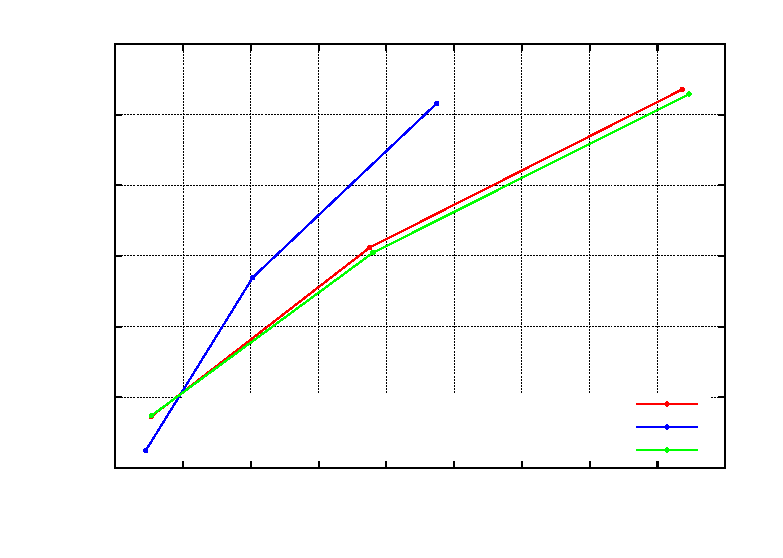
\includegraphics{1}}%
    \gplfronttext
  \end{picture}%
\endgroup

    \caption{Configuraties kwaliteitsschaalbaarheid}
    \label{graph:graph1}
  \end{center}
\end{figure}
We merken op dat SVC met inter-layer predictie duidelijk veel beter presteert dan een simulcast van single layers of een SVC zonder inter-layer predictie. Bij een multicast van single layers zal een betere kwaliteit single-layer opnieuw de basisinfo bevatten die ook in een lagere kwaliteit single-layer zit. Zo wordt er dus veel info dubbel opgeslaan. De multicast van single layers en de SVC zonder inter-layerpredictie zijn ongeveer even effici\"ent.
\section{Spatiale schaalbaarheid}
We maakten eerst een geschaalde versie van \verb$BBB_640x360_24.yuv$ aan met het commando
\begin{verbatim}
DownconvertStatic.exe 640 360 BBB_640x360_24.yuv 320 180 BBB_320x180_12.yuv
\end{verbatim}
De PSNR waarden werden berekend zoals besproken in de vorige opgave.
\begin{figure}[H]
  \begin{center}
    % GNUPLOT: LaTeX picture with Postscript
\begingroup
  \makeatletter
  \providecommand\color[2][]{%
    \GenericError{(gnuplot) \space\space\space\@spaces}{%
      Package color not loaded in conjunction with
      terminal option `colourtext'%
    }{See the gnuplot documentation for explanation.%
    }{Either use 'blacktext' in gnuplot or load the package
      color.sty in LaTeX.}%
    \renewcommand\color[2][]{}%
  }%
  \providecommand\includegraphics[2][]{%
    \GenericError{(gnuplot) \space\space\space\@spaces}{%
      Package graphicx or graphics not loaded%
    }{See the gnuplot documentation for explanation.%
    }{The gnuplot epslatex terminal needs graphicx.sty or graphics.sty.}%
    \renewcommand\includegraphics[2][]{}%
  }%
  \providecommand\rotatebox[2]{#2}%
  \@ifundefined{ifGPcolor}{%
    \newif\ifGPcolor
    \GPcolorfalse
  }{}%
  \@ifundefined{ifGPblacktext}{%
    \newif\ifGPblacktext
    \GPblacktexttrue
  }{}%
  % define a \g@addto@macro without @ in the name:
  \let\gplgaddtomacro\g@addto@macro
  % define empty templates for all commands taking text:
  \gdef\gplbacktext{}%
  \gdef\gplfronttext{}%
  \makeatother
  \ifGPblacktext
    % no textcolor at all
    \def\colorrgb#1{}%
    \def\colorgray#1{}%
  \else
    % gray or color?
    \ifGPcolor
      \def\colorrgb#1{\color[rgb]{#1}}%
      \def\colorgray#1{\color[gray]{#1}}%
      \expandafter\def\csname LTw\endcsname{\color{white}}%
      \expandafter\def\csname LTb\endcsname{\color{black}}%
      \expandafter\def\csname LTa\endcsname{\color{black}}%
      \expandafter\def\csname LT0\endcsname{\color[rgb]{1,0,0}}%
      \expandafter\def\csname LT1\endcsname{\color[rgb]{0,1,0}}%
      \expandafter\def\csname LT2\endcsname{\color[rgb]{0,0,1}}%
      \expandafter\def\csname LT3\endcsname{\color[rgb]{1,0,1}}%
      \expandafter\def\csname LT4\endcsname{\color[rgb]{0,1,1}}%
      \expandafter\def\csname LT5\endcsname{\color[rgb]{1,1,0}}%
      \expandafter\def\csname LT6\endcsname{\color[rgb]{0,0,0}}%
      \expandafter\def\csname LT7\endcsname{\color[rgb]{1,0.3,0}}%
      \expandafter\def\csname LT8\endcsname{\color[rgb]{0.5,0.5,0.5}}%
    \else
      % gray
      \def\colorrgb#1{\color{black}}%
      \def\colorgray#1{\color[gray]{#1}}%
      \expandafter\def\csname LTw\endcsname{\color{white}}%
      \expandafter\def\csname LTb\endcsname{\color{black}}%
      \expandafter\def\csname LTa\endcsname{\color{black}}%
      \expandafter\def\csname LT0\endcsname{\color{black}}%
      \expandafter\def\csname LT1\endcsname{\color{black}}%
      \expandafter\def\csname LT2\endcsname{\color{black}}%
      \expandafter\def\csname LT3\endcsname{\color{black}}%
      \expandafter\def\csname LT4\endcsname{\color{black}}%
      \expandafter\def\csname LT5\endcsname{\color{black}}%
      \expandafter\def\csname LT6\endcsname{\color{black}}%
      \expandafter\def\csname LT7\endcsname{\color{black}}%
      \expandafter\def\csname LT8\endcsname{\color{black}}%
    \fi
  \fi
  \setlength{\unitlength}{0.0500bp}%
  \begin{picture}(7200.00,5040.00)%
    \gplgaddtomacro\gplbacktext{%
      \csname LTb\endcsname%
      \put(1078,704){\makebox(0,0)[r]{\strut{} 37}}%
      \csname LTb\endcsname%
      \put(1078,1156){\makebox(0,0)[r]{\strut{} 37.5}}%
      \csname LTb\endcsname%
      \put(1078,1609){\makebox(0,0)[r]{\strut{} 38}}%
      \csname LTb\endcsname%
      \put(1078,2061){\makebox(0,0)[r]{\strut{} 38.5}}%
      \csname LTb\endcsname%
      \put(1078,2513){\makebox(0,0)[r]{\strut{} 39}}%
      \csname LTb\endcsname%
      \put(1078,2966){\makebox(0,0)[r]{\strut{} 39.5}}%
      \csname LTb\endcsname%
      \put(1078,3418){\makebox(0,0)[r]{\strut{} 40}}%
      \csname LTb\endcsname%
      \put(1078,3870){\makebox(0,0)[r]{\strut{} 40.5}}%
      \csname LTb\endcsname%
      \put(1078,4323){\makebox(0,0)[r]{\strut{} 41}}%
      \csname LTb\endcsname%
      \put(1078,4775){\makebox(0,0)[r]{\strut{} 41.5}}%
      \csname LTb\endcsname%
      \put(1210,484){\makebox(0,0){\strut{} 100}}%
      \csname LTb\endcsname%
      \put(1909,484){\makebox(0,0){\strut{} 150}}%
      \csname LTb\endcsname%
      \put(2608,484){\makebox(0,0){\strut{} 200}}%
      \csname LTb\endcsname%
      \put(3307,484){\makebox(0,0){\strut{} 250}}%
      \csname LTb\endcsname%
      \put(4007,484){\makebox(0,0){\strut{} 300}}%
      \csname LTb\endcsname%
      \put(4706,484){\makebox(0,0){\strut{} 350}}%
      \csname LTb\endcsname%
      \put(5405,484){\makebox(0,0){\strut{} 400}}%
      \csname LTb\endcsname%
      \put(6104,484){\makebox(0,0){\strut{} 450}}%
      \csname LTb\endcsname%
      \put(6803,484){\makebox(0,0){\strut{} 500}}%
      \put(176,2739){\rotatebox{-270}{\makebox(0,0){\strut{}PSNR-Y [dB]}}}%
      \put(4006,154){\makebox(0,0){\strut{}Bitrate [kbps]}}%
    }%
    \gplgaddtomacro\gplfronttext{%
      \csname LTb\endcsname%
      \put(5816,1317){\makebox(0,0)[r]{\strut{}Single-layer codering}}%
      \csname LTb\endcsname%
      \put(5816,1097){\makebox(0,0)[r]{\strut{}SVC met inter-layer predictie}}%
      \csname LTb\endcsname%
      \put(5816,877){\makebox(0,0)[r]{\strut{}SVC zonder inter-layer predictie}}%
    }%
    \gplbacktext
    \put(0,0){
\includegraphics{2}}%
    \gplfronttext
  \end{picture}%
\endgroup

    \caption{Configuraties spatiale schaalbaarheid}
    \label{graph:graph1}
  \end{center}
\end{figure}
\noindent Als we kijken naar de punten van de single-layer, zien we dat die veel beter presteert dan de SVC. Dit komt omdat single-layer het minst informatie bevat. We vinden het raar dat SVC zonder inter-layer predictie beter presteert dan met.
\end{document}